%!TEX encoding = UTF-8 Unicode
\documentclass[a4paper]{report}
\usepackage[utf8]{inputenc}
\usepackage[a4paper, left=3cm, right=0.5 cm, top=0.5cm, bottom=0.5cm]{geometry}
\usepackage{graphicx}

\setcounter{tocdepth}{2}

\begin{document}
\title{Hardware implementation report}
\author{Igor Chudov}
\date{April 2019}
\maketitle

\begin{abstract}
The document describes the networking environment and end-user device
operation and restrictions for the project.
\end{abstract}

\part{Project analysis}

\chapter{User story}

I'm a kid older than 3. I'm in a pre-school or elementary-school age. I
have a tablet computer provided only for educational purposes. I use a
computer mostly at school but I can take it home for the weekend. I may
be not very experienced with computers but I have lots of time, energy
and curiosity. \\

\noindent
I'm using my device in a network set up like: \\*
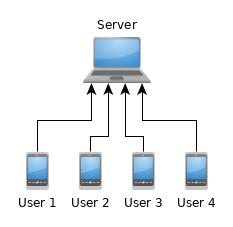
\includegraphics{school.png}


\chapter{Known issues and limitations}

\begin{itemize}
\item The end-user device must be cheaper than \$ 100.
\item The device will work in untrusted environment: at home, for example.
\end{itemize}


\chapter{Goals}

\begin{enumerate}
\item Provide a cheap replaceable device for educational purposes.
\item Determine the project hardware equpment and networking environment.
\end{enumerate}


\chapter{Scope of work}

\section{Requirements}

\begin{enumerate}
\item The end-user device must have a simple rollback functionality for
the cases of incorrect user exploitation.
\item The end-user device must have a limited access to the websites.
\item The end-user device must have application installation
functionality blocked.
\end{enumerate}

\section{Defintion of Done (artifacts)}

\begin{enumerate}
\item Report describing solutions for limiting access to websites and
3rd party software on end-user devices.
\item Provide simple device configuration tutorial in english
\textbf{or} spanish.
\end{enumerate}


\part{Project state}

\chapter{Overview}

There were two devices used for testing and investigation:
\textbf{Lenovo TB-7304i} and \textbf{Alldocube T1006S}. The devices
tested had notable differences in Android OS configurations so it
will be hard to maintain the same level of functionality across
different hardware models.

\chapter{Server-side}

Devices may be configured via \textbf{ADB over Wi-Fi} after some initial
setup and that functionality may be useful for configuration deployment
on multiple machines, but this case needs more investigation.

This functionality may be used not only for initial deployment but also
for massive device reset/rollback without interaction with users.

\chapter{Client-side}

Generally, standard parental control function is enough to provide the
necessary security level for children. Currently the configuration
process is manual and there is no way provided to ensure that multiple
devices will be configured alike.

Unfortunately \textbf{Alldocube T1006S} model provided had
\textbf{"Restricted profile"} functionality turned off making it
unsuitable for the task in device's unmodified state.


\chapter{Risks}

\begin{itemize}
\item \textbf{Current model with supposed software and/or user reset
done by a person won't work} because each setup takes lots of time and
is error-prone. This will lead to numerous setup errors and the project
will have all chances to stop because of this.
\item \textbf{There is a need for a single device model} because different
models from different vendors differs too much. This will lead to
growth of instructions, workarounds, tests and incur numerous problems
for product developers.
\item \textbf{Tests on Lenovo TB-7304i shown that Google Chrome is
inaccessible for Restricted Profiles} so the developers will have to
test the product with Android's \textbf{"Safe Browser"}. The problem
may be solved by lower-level Android OS configuration but this case
needs more investigation.
\end{itemize}


\part{Project details}

\chapter{Server side}

It's advised to have as much functionality on server-side as possible
to reduce problems with client devices.


\section{Authentication}

There is software for WiFi HotSpots fencing called \textbf{CoovaChilli}:
http://coova.github.io/CoovaChilli/ . It's abandoned somehow but it's
the most functional solution for organizing fenced connection of
multiple users.


\section{Authorization}

Tasks like filtering the undesired traffic are also done better from
the server side - it'll be possible to avoid such problems like
adjusting tablets for this kind of work.


\chapter{End user side}

It's expected that the target audience is totally inexperienced with
computers so the less actions they will need to do to achieve the
desired result - the better.


\section{Access limiting}

Android's standard profiles and parental control function is enough to
limit the end-user access to programs and whitelisted websites.

The account of the device owner may be protected by graphical key
making it rather problematic to crack.

It should also be noted that modern Android versions have device control
feature that may prevent the unauthorized user from device reset -
in case the device reset is performed without correct password - the
device may turn into brick and become nearly irreparable (may be
solved only by reflashing new OS on device).

The setup is point-and-click as for now so it won't work in case of
hundreds and thousands of devices but there is some ways (like using
Termux with configuration deployment tools) which must be investiated
further.


\subsection{Note on bypassing parental control function}

The problem boils down to graphical key bypass. There are
several ways to do it:

\begin{enumerate}
\item \textbf{Finding a graphical key}
The device inspected (Lenovo TB-7304i) had unlimited amount of
graphical key tries. The device makes 30-second pause each 10 tries.

It's possible to guess the key by inspecting traces left by fingers.
There are not very many variants of graphical key the user may remember
\item \textbf{Hard reset}
\item \textbf{Remote unblock using Google account}
It's possible to unblock the device remotely in case the Google account
is accessible.
\item \textbf{Nonstandard ways}
The user will have to preinstall special applications first.
\end{enumerate}


\section{Authentication}

Done transparently when device is connected to HotSpot via MAC. The
authentication and authorization is performed by CoovaChilli software
on server side.


\section{Rollbacks}

Android's new filesystem F2FS has snapshot and rollback functionality
but it must be investigated if it's used by existing devices.


\section{Threat model}

There is two kind of threats we expect:

\begin{enumerate}
\item Treats from external network: miners, viruses, etc.
\item Treats from users: curios children
\end{enumerate}

Here is the list of treats we're trying to mitigate:

\begin{itemize}
\item Getting full control on device by its end-user.
\item Getting sensitive personal information from device's
\textbf{"Emergency Information"}.
\end{itemize}


\end{document}

